\documentclass[a4paper,titlepage]{article}
\usepackage[utf8]{inputenc}
\usepackage{fullpage}
\usepackage{indentfirst}
\usepackage[per-mode=symbol]{siunitx}
\usepackage{listings}
\usepackage{graphicx}
\usepackage{color}
\usepackage{amsmath}
\usepackage{mathtools}
\usepackage{array}
\usepackage[hidelinks]{hyperref}
\usepackage[format=plain,font=it]{caption}
\usepackage{subcaption}
\usepackage{standalone}
\usepackage[nottoc]{tocbibind}
\usepackage[noabbrev,capitalize,nameinlink]{cleveref}
\usepackage{listings}
\usepackage{xspace}
\usepackage{tikz}
\usepackage{circuitikz}
\usepackage{titlesec}
\usepackage[cache=false]{minted}
\usepackage{booktabs}
\usepackage{csvsimple}
\newcommand{\MATLAB}{\textsc{Matlab}\xspace}
\usepackage{siunitx}
\usepackage[super]{nth}
\usepackage[titletoc]{appendix}

% Custom commands
\newcommand\numberthis{\addtocounter{equation}{1}\tag{\theequation}}
\newcommand{\code}[1]{\texttt{#1}}
\newcolumntype{P}[1]{>{\centering\arraybackslash}p{#1}}

\tikzstyle{my help lines}=[gray,thick,dashed]

\setminted{linenos,breaklines,fontsize=auto}

%\titleformat*{\section}{\normalsize\bfseries}
%\titleformat*{\subsection}{\small\bfseries}
\renewcommand{\thesubsection}{\thesection.\alph{subsection}}
\providecommand*{\listingautorefname}{Listing}
\newcommand*{\Appendixautorefname}{Appendix}

%opening
\title{\textbf{ECSE 543: Numerical Methods} \\ Assignment 2 Report}
\author{Wenjie Wei \\ 260685967}
\date{\today}

\begin{document}
	\sloppy
	\maketitle
	
	\tableofcontents
	\newpage
	
	\section*{Introduction}
		In this assignment, three numerical methods discussed in class were explored. The interpreter used for the Python codes is Python 3.6. 
		
	\section{First Order Finite Element Problem}
		Figure \ref{prob} shows an illustration of the first order triangular finite element problem to be solved. 
		\begin{figure}[!h]
			\centering
			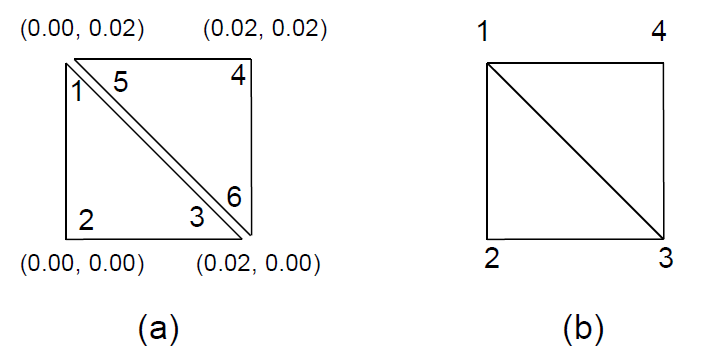
\includegraphics[width=0.7\linewidth]{prob}
			\caption{1st Order Triangular FE Problem}
			\label{prob}
		\end{figure}
	
		Take the triangle with nodes 1, 2, and 3 as the beginning step. Firstly, interpolate the potential \textit{U} as:
		$$
			U = a + bx + cy
		$$
		and at vertex 1, we can write an equation of potential as:
		$$
			U_1 = a + bx_1 + cy_1
		$$
		
		Thus, we can have a vector of potentials for vertex 1, 2, and 3 as follows:
		$$
			\begin{bmatrix}
				U_1 \\ U_2 \\ U_3
			\end{bmatrix} = 
			\begin{bmatrix}
				1 & x_1 & y_1 \\
				1 & x_2 & y_2 \\
				1 & x_3 & y_3 
			\end{bmatrix}
			\begin{bmatrix}
				a \\ b \\ c
			\end{bmatrix}
		$$
		and the terms $a, b, c$ are acquired following:
		\begin{equation}
			U = \sum_{i = 1}^{3} U_i\alpha_i(x, y)
		\end{equation}
		and we can derive a general formula for $\alpha_i$:
		\begin{equation}
			\nabla \alpha_i = \nabla \frac{1}{2A}[(x_{i+1}y_{i+2}-x_{i+2}y_{i+1}) + (y_{i+1}-y_{i+2})x+(x_{i+2}-x_{i+1})y]			
		\end{equation}
		where $A$ holds the value of the area of the triangle.
		
		Following Equation 2, when the index $i$ exceeds the top limit 3, it is wrapped around to 1. Now we can get the following calculations for $\alpha_1$, $\alpha_2$ and $\alpha_3$:
		$$
			\nabla \alpha_1 = \nabla \frac{1}{2A}[(x_2y_3-x_3y_2) + (y_2-y_3)x+(x_3-x_2)y]
		$$
		$$
			\nabla \alpha_2 = \nabla \frac{1}{2A}[(x_3y_1-x_1y_3) + (y_3-y_1)x+(x_1-x_3)y]
		$$
		$$
			\nabla \alpha_3 = \nabla \frac{1}{2A}[(x_1y_2-x_2y_1) + (y_1-y_2)x+(x_2-x_1)y]
		$$
		
		With the expressions for $\alpha$ derived, we now go ahead and calculate the \textbf{$S_{ij}^{(e)}$} matrices. The general formula below is used to calculate the \textbf{\textit{S}} matrix:
		\begin{equation}
			S^{(e)}_{ij} = \int_{\Delta e} \nabla \alpha_i \nabla \alpha_j dS
		\end{equation}
		
		Using the equation above, plug in the values provided in Figure \ref{prob}, we can have the following calculations:
		$$
			S_{11} = \frac{1}{4A}[(y_2 - y_3)^2 + (x_3 - x_2)^2] = \frac{1}{4 \times 2 \times 10^{-4}}[0 + 0.02^2] = 0.5
		$$
		$$
			S_{12} = \frac{1}{4A}[(y_2 - y_3)(y_3 - y_1) + (x_3 - x_2)(x_1 - x_3)] = -0.5
		$$
		$$
			S_{13} = \frac{1}{4A}[(y_2 - y_3)(y_1 - y_2) + (x_3 - x_2)(x_2 - x_1)] = 0
		$$
		
		Before performing the calculation for the next row, we inspect the calculation rules of the entries of the \textbf{\textit{S}} matrix, we can easily discover that $S_{ij} = S_{ji}$, since the flip of the orders of the operands in the parenthesis results in the same sign of the result. Therefore, the following statements can be made:
		$$
			S_{21} = S_{12} = -0.5
		$$
		$$
			S_{31} = S_{13} = 0
		$$
		
		$$
			S_{22} = \frac{1}{4A}[(y_3 - y_1)^2 + (x_1 - x_3)^2] = 1
		$$
		$$
			S_{23} = S_{32} = \frac{1}{4A}[(y_3 - y_1)(y_1 - y_2) + (x_1 - x_3)(x_2 - x_1)] = -0.5
		$$
		$$
			S_{33} = \frac{1}{4A}[(y_1 - y_2)^2 + (x_2 - x_1)^2] = 0.5
		$$
		
		From the calculation results above, we can come up with the \textbf{\textit{S}} matrix for vertices 1, 2, and 3:
		$$
			S^{(1)} = \begin{bmatrix}
				S_{11} & S_{12} & S_{13}\\
				S_{21} & S_{22} & S_{23} \\
				S_{31} & S_{32} & S_{33} \\
			\end{bmatrix} = 
			\begin{bmatrix}
				0.5 & -0.5 & 0\\
				-0.5 & 1 & -0.5 \\
				0 & -0.5 & 0.5
			\end{bmatrix}
		$$
		
		Use the similar approach for the other triangle and obtain $S_{456}$:
		$$
			S^{(2)} = \begin{bmatrix}
				S_{44} & S_{45} & S_{46}\\
				S_{54} & S_{55} & S_{56} \\
				S_{64} & S_{65} & S_{66} \\
			\end{bmatrix} = 
			\begin{bmatrix}
				1 & -0.5 & -0.5\\
				-0.5 & 0.5 & 0 \\
				-0.5 & 0 & 0.5
			\end{bmatrix}
		$$
		
		Add the triangles to get the energy of the whole system shown in (b) of Figure \ref{prob}:
		$$
			\begin{bmatrix}
				U_1 \\
				U_2 \\
				U_3 \\
				U_4 \\
				U_5 \\
				U_6				
			\end{bmatrix}_{dis} = 
			\begin{bmatrix}
				1&&&\\
				&1&&\\
				&&1&\\
				&&&1\\
				1&&&\\
				&&1&
			\end{bmatrix}
			\begin{bmatrix}
				U_1 \\
				U_2 \\
				U_3 \\
				U_4
			\end{bmatrix}_{joint}
		$$
		which is also denoted as:
		$$
			U_{dis} = CU_{joint}
		$$
		
		Use $\textbf{S}_{dis}$ to denote a $6\times 6$ matrix to represent the disjoint matrix:
		$$
			S_{dis} = 
			\begin{bmatrix}
				S^{(1)} & \\
				 & S^{(2)}				
			\end{bmatrix} = 
			\begin{bmatrix}
				0.5 & -0.5 & 0 & & & \\
				-0.5 & 1 & -0.5 & & & \\
				0 & -0.5 & 0.5 & & & \\
				& & & 1 & -0.5 & -0.5 \\
				& & & -0.5 & 0.5 & 0 \\
				& & & -0.5 & 0 & 0.5
			\end{bmatrix}
		$$
		
		Now the global \textbf{\textit{S}} matrix will be calculated as:
		\begin{align*}
			S_{joint} &= C^TS_{dis}C \\
			&= 
			\begin{bmatrix}
				1&&&&1&\\
				&1&&&&\\
				&&1&&&1\\
				&&&1&&
			\end{bmatrix}
			\begin{bmatrix}
				0.5 & -0.5 & 0 & & & \\
				-0.5 & 1 & -0.5 & & & \\
				0 & -0.5 & 0.5 & & & \\
				& & & 1 & -0.5 & -0.5 \\
				& & & -0.5 & 0.5 & 0 \\
				& & & -0.5 & 0 & 0.5
			\end{bmatrix}
			\begin{bmatrix}
				1&&&\\
				&1&&\\
				&&1&\\
				&&&1\\
				1&&&\\
				&&1&
			\end{bmatrix}\\
			&= \begin{bmatrix}
				1 & -0.5 & 0 & -0.5\\
				-0.5 & 1 & -0.5 & 0\\
				0 & -0.5 & 1 & -0.5\\
				-0.5 & 0 & -0.5 & 1
			\end{bmatrix}
		\end{align*}
		which is the final result of this problem.
	\section{Coaxial Cable Electrostatic Problem}
		Use the triangular finite element model for the analysis of the coaxial cable problem seen in the previous assignment. We take the third quadrant for the analysis. 
		\subsection{The Finite Element Mesh}
			Listing \ref{lst:finite_element} shows the implementation of the construction of the finite element mesh and the creation of the \MATLAB input file.
			\begin{figure}[!h]
				\centering
				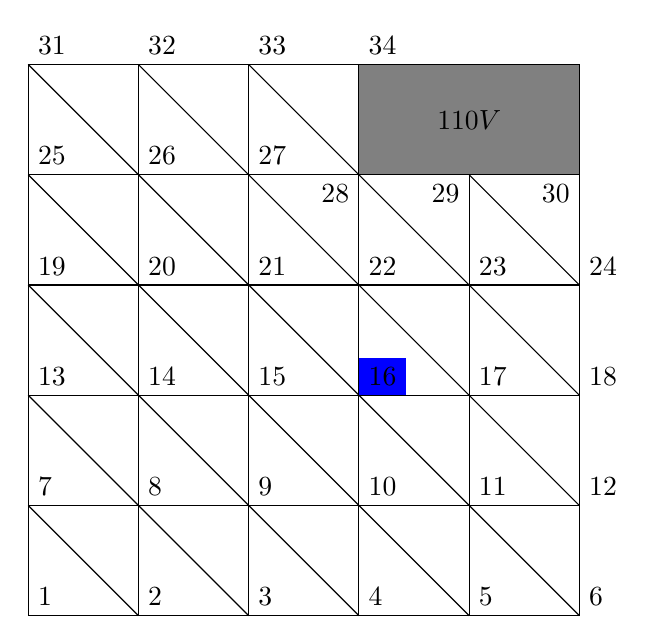
\begin{tikzpicture}[scale=1.4]
					\draw (0, 0) grid (5, 4);
					\draw (0,1) -- (1,0);
					\draw (0,2) -- (2,0);
					\draw (0,3) -- (3,0);
					\draw (0,4) -- (4,0);
					\draw (0,4) grid (3,5);
					\draw (0,5) -- (5,0);
					\draw (1,5) -- (5,1);
					\draw (2,5) -- (5,2);
					\draw (4,4) -- (5,3);
					\draw [fill=gray] (3,4) rectangle (5,5);					
					\node at (4, 4.5) {$110V$};
					\node[above right] at (0,0) {$1$};
					\node[above right] at (1,0) {$2$};
					\node[above right] at (2,0) {$3$};
					\node[above right] at (3,0) {$4$};
					\node[above right] at (4,0) {$5$};
					\node[above right] at (5,0) {$6$};
					\node[above right] at (0,1) {$7$};
					\node[above right] at (1,1) {$8$};
					\node[above right] at (2,1) {$9$};
					\node[above right] at (3,1) {$10$};
					\node[above right] at (4,1) {$11$};
					\node[above right] at (5,1) {$12$};
					\node[above right] at (0,2) {$13$};
					\node[above right] at (1,2) {$14$};
					\node[above right] at (2,2) {$15$};
					\node[fill=blue,above right] at (3,2) {$16$};
					
					\node[above right] at (4,2) {$17$};
					\node[above right] at (5,2) {$18$};
					\node[above right] at (0,3) {$19$};
					\node[above right] at (1,3) {$20$};
					\node[above right] at (2,3) {$21$};
					\node[above right] at (3,3) {$22$};
					\node[above right] at (4,3) {$23$};
					\node[above right] at (5,3) {$24$};
					\node[above right] at (0,4) {$25$};
					\node[above right] at (1,4) {$26$};
					\node[above right] at (2,4) {$27$};
					\node[below left] at (3,4) {$28$};
					\node[below left] at (4,4) {$29$};
					\node[below left] at (5,4) {$30$};
					\node[above right] at (0,5) {$31$};
					\node[above right] at (1,5) {$32$};
					\node[above right] at (2,5) {$33$};
					\node[above right] at (3,5) {$34$};
				\end{tikzpicture}
				\caption{Organization of the Finite Element Mesh}
				\label{fe_mesh_fig}
			\end{figure}
		
			Figure \ref{fe_mesh_fig} shows the organization of the finite element mesh constructed by the program. The input file written by this program is shown in Listing \ref{lst:SIMPLE2D.dat}. Note that the first number at the beginning of the lines are not an input to the \MATLAB file, as it is the line number which is provided by the \textit{minted} package in \LaTeX. 
			
		\subsection{Potential Solved by SIMPLE2D.m}
			Use the input file generated in the previous section, we are able to use the \MATLAB file to calculate the potential at every node we have specified. The output of the SIMPLE2D.m file is shown in Listing \ref{lst:potential.dat}. The target node (0.06, 0.04) is highlighted in blue as Node 16, and from Listing \ref{lst:potential.dat} shows that the potential at this node is $40.527V$.
			
		\subsection{Capacitance per Unit Length}
			To compute the capacitance, apply the fundamental Equation \ref{capacitance}: 
			\begin{equation}
				E = \frac{1}{2} CV^2
				\label{capacitance}
			\end{equation}
			
			Now apply the finite element method used in the previous section. Use $U_{joint}$ to denote the potential vector shown in Listing \ref{lst:potential.dat}. Use the $S_{joint}$ calculated in the first question, we derive an equation to calculate the total capacitance:
			\begin{equation}
				E = \frac{1}{2}\varepsilon_0 U^T_{joint}S_{joint}U{joint}
			\end{equation}
			
	\newpage
	\begin{appendices}
		
		\section{Code Listings} \label{appendix:code}
		
		\setminted{linenos,breaklines,fontsize=\footnotesize}
		
		\begin{center}
			\captionof{listing}{Finite Element Mesh Implementation (\texttt{finite\_element.py}).}
			\inputminted{python}{../finite_element.py}
			\label{lst:finite_element}
		\end{center}
		
		\newpage
		\twocolumn
		\begin{center}
			\captionof{listing}{Finite Element Mesh Input File}
			\inputminted{python}{../SIMPLE2Dinput.dat}
			\label{lst:SIMPLE2D.dat}
		\end{center}
	
		\begin{center}
			\captionof{listing}{\MATLAB File Outputs}
			\inputminted{python}{../potentials.dat}
			\label{lst:potential.dat}
		\end{center}
		\newpage
		
	\end{appendices}
	
\end{document}